\section{Holistic Indexing}
\label{sec:problem}

In this section we discuss the fundamentals of holistic indexing.
We designed holistic indexing on top of column-store architectures inspired by their flexibility on manipulating some attributes without affecting the rest.
During query processing indices are built and optimized incrementally by adapting to query predicates, as in adaptive indexing.
However, in contrast to adaptive indexing, index refinement actions are not triggered only as a side-effect of query processing; 
in holistic indexing incremental index optimization actions take place continuously in order to exploit 
under-utilized CPU cores. Thus, concurrently with user queries, system queries also refine the index space.
Holistic indexing monitors the workload and CPU resources utilization and every time it detects that the system is under-utilized
it exploits statistical information to decide which indices to refine and by how much. 

Thus, with holistic indexing we achieve an always active 
self-organizing DBMS by continuously adjusting the physical design to workload demands.

\vspace{2mm}
\emph{\textbf{Problem Definition:} Given a set of adaptive indices, statistical information about the past workload, storage constraints and the CPU utilization, continuously select indices from the index space and incrementally refine them, while the materialized index space size does not exceed the storage budget.}
\vspace{2mm}

In the rest of this section, we discuss in detail how we fit holistic indexing in a modern DBMS architecture. 

\subsection{Preliminary Definitions}
\label{subsec:definitions}

First, we give a series of definitions.

\textbf{Workload.} A workload \emph{W} consists of a sequence of user queries, inserts and deletes. Updates are translated into a deletion that is followed by an insertion.

\textbf{CPU Utilization.} CPU utilization in a time interval $dt$ describes how much of the available CPU power is used in $dt$. Specifically, it expresses the percentage of total CPU time, i.e., the amount of time for which the CPU is used for processing user or kernel processes instead of being idle. CPU utilization is calculated using (operating system) kernel statistics.

\textbf{Configuration.} A configuration is defined as a set of adaptive indices that can be used in the physical design.
There are three kinds of configurations.
The \emph{actual configuration}, \emph{C$_{actual}$}, contains indices on attributes that have already been accessed by user queries in the workload.
Indices are inserted in \emph{C$_{actual}$} when they are created during query processing.
For instance, assume a query $Q$ enters the system and contains a selection on an attribute $A$.
If the adaptive index on $A$ does not exist, it is created on-the-fly and it is inserted in \emph{C$_{actual}$}.

Besides \emph{C$_{actual}$}, holistic indexing also maintains the \emph{potential configuration}. \emph{C$_{potential}$},
 which contains indices on attributes that have not been queried yet.
Indices are inserted in \emph{C$_{potential}$} either automatically by the system or manually by the user.
Finally, the \emph{optimal configuration}, \emph{C$_{optimal}$}, contains indices that have reached the optimal status (the next paragraph describes when an index is considered optimal).
The union of \emph{C$_{actual}$} and \emph{C$_{potential}$} constitutes the index space \emph{IS}, i.e., the indices which are candidates for
incremental optimization when the system is under-utilized.
Later, in Section~\ref{subsec:design}, we describe how the system is educated to pick an index from \emph{IS}.
Indices from \emph{C$_{optimal}$} are not considered for further refinement during the physical design reorganization.

\textbf{Optimal Index.} 
Holistic indexing exploits adaptive indices.
As seen in Section~\ref{subsec:cracking}, an adaptive index is refined during query 
processing by physically reorganizing pieces of the cracker column based on query predicates.
As more queries arrive, more pieces are created, and thus, the pieces become smaller.
We have found that when the size of the pieces becomes equal to L$_{1}$ cache size ($|L_1|$), further refinements are not necessary;
a smaller size increases administration costs to maintain the extra pieces and it does not bring any significant extra benefit as scanning inside L$_{1}$ is fast anyway (no cache misses).
Pieces of size smaller than L$_{1}$ cache can either be sorted 
or queries simply need to scan them (a range select operator has to scan at most two L$_{1}$ pieces).
An index \emph{I} on an attribute $A$ is considered optimal (\emph{I$_{opt}$}), 
when the average size of pieces ($|p|$) in $A_{CRK}$ is equal to the size of L$_{1}$ cache.
Equation \eqref{eq:d} describes the distance between \emph{I} and \emph{I$_{opt}$}.
\vspace{-0.25em}
\begin{equation}
d(I,I_{opt}) = |p| -|L_{1}| = \frac{N_A}{p_A} - |L_{1}|
\label{eq:d}
\vspace{-0.25em}
\end{equation}

$N_A$ is the total number of tuples in $A_{CRK}$ while $p_A$ is the total number of pieces in $A_{CRK}$.
This information is readily available and thus we can easily calculate the average piece size
in a cracker column and in turn we can calculate the distance of the respective cracker index from its optimal status.

\textbf{Statistical Information.} 
During query processing holistic indexing continuously monitors the workload and the CPU utilization.
For each column in the schema it collects information regarding how many times it has been accessed by user queries,
how many pieces the relevant cracker column contains, how many queries did not need to further refine the index
because there was an exact hit.
Besides the statistical information about the workload, kernel statistics are used in order to monitor the CPU utilization.


%\newpage
\subsection{System Design}
\label{subsec:design}

Holistic indexing is always active.
It continuously monitors the workload and the CPU utilization.
When under-utilized CPU cores are detected, holistic indexing exploits them in order to adjust the physical design based
on the collected statistical information.
The system performs several index refinement steps simultaneously depending on available CPU resources. 
Everything happens in parallel to query processing, but without disturbing running queries.


We discuss in detail the continuous tuning process and how to exploit under-utilized CPU cycles. We also discuss how existing adaptive indexing solutions on %
 core database architectures issues%
 such as updates and concurrency control can be directly adapted to work with holistic indexing.


\textbf{Statistics per Column/Index.}
Statistics per column are collected during query processing.
This is the job of the select operator as it is within the select operator that all (user query) 
adaptive indexing actions take place.  
Every time an attribute is accessed for a selection of a user query, the select operator
updates a data structure, which contains all statistics for the respective index.
Given that the select operator performs adaptive indexing actions anyway,
it already has access to critical information such as how many new pieces were created 
during new cracking actions for this query,
whether the select was an exact match, etc.
All information is stored in a heap structure (one node per index) 
which allows us to easily put new indices in the configuration or drop old ones.
The structure is protected with read/write latches as multiple queries  or holistic workers (discussed later on) 
may be cracking in parallel.


\textbf{Tuning Cycle.} 
At all times there is an active \emph{holistic indexing thread} which runs in parallel to user queries.
The responsibility of the holistic indexing thread is to monitor the CPU utilization and to activate \emph{holistic worker threads} 
to perform auxiliary index refinement actions whenever idle CPU cycles are detected.
The tuning process is shown in Figure~\ref{fig:diagram}.
The holistic indexing thread continuously monitors the CPU load at intervals of  $1$ second at a time.
In case holistic worker threads are activated, the holistic indexing thread waits for all worker threads to finish and measures the CPU utilization within the next $1$ second. 
In our analysis, we found that $1$ second is the time limit that gives proper kernel statistics.
%In addition, while the worker threads are activated, we do not measure the CPU utilization in order to avoid including the CPU power consumed by the worker threads. 
When $n$ idle CPU cores are detected, $n$ holistic worker threads are activated.
Each worker thread executes an instance of the IdleFunction, which picks an index from the Index Space $IS$ and performs $x$ 
partial index refinement actions on it.
Every time an index is refined, the respective statistics, e.g., distance from the optimal index, are updated.
When an index reaches the optimal status, it is moved into the optimal configuration \emph{C$_{optimal}$}.

A side-effect of the tuning process is that some of the holistic worker threads might remain idle while the holistic indexing thread waits for all workers to finish.
However, as we show later in Section~\ref{subsec:motivation} (Figure~\ref{fig:motiv}(d)), this happens only for very short periods of time and as 
the system adapts to the workload this phenomenon disappears (as the pieces queried in the adaptive indices become smaller and smaller 
the holistic indexing workers end up doing tasks of similar weight as none is going to touch a very big piece).


\textbf{Index Refinement.}
Every time a worker thread wakes up, it performs $x$ index refinements on a single column. $x$ is a tuning parameter. 
In our analysis in Section~\ref{subsec:decisions} (Figure~\ref{fig:cracks_number}) we found that a good value for our hardware set-up is $x=16$. 
The index refinements are performed by picking $x$ random values in the domain of the respective
attribute and cracking the column based on these values. In this way, each time a worker thread cracks a single
piece of a column it splits this piece into two new pieces based on the pivot. 

There are numerous choices on how to choose a pivot. We found that picking a random pivot is the most cost efficient choice.
Other options include to crack the biggest piece of the column, i.e., with the rationale that this takes more work out of future queries.
Another option is to crack the smallest piece, i.e., with the rationale that this piece is small because it is hot (because many queries access it for cracking).
However, such options are hard to achieve in a lightweight way as we need to maintain a structure such as  a priority queue
to know which piece is the biggest or smallest every time. 
Since every cracking action costs a few microseconds or milliseconds it is not worth the extra storage and CPU cost to maintain auxiliary structures.
Random pivots converge quickly to cracking the whole domain,
providing a column which is balanced in terms of which pieces are cracked
and requiring no extra costs in deciding which pivot to choose. 


\begin{figure}
\begin{center}
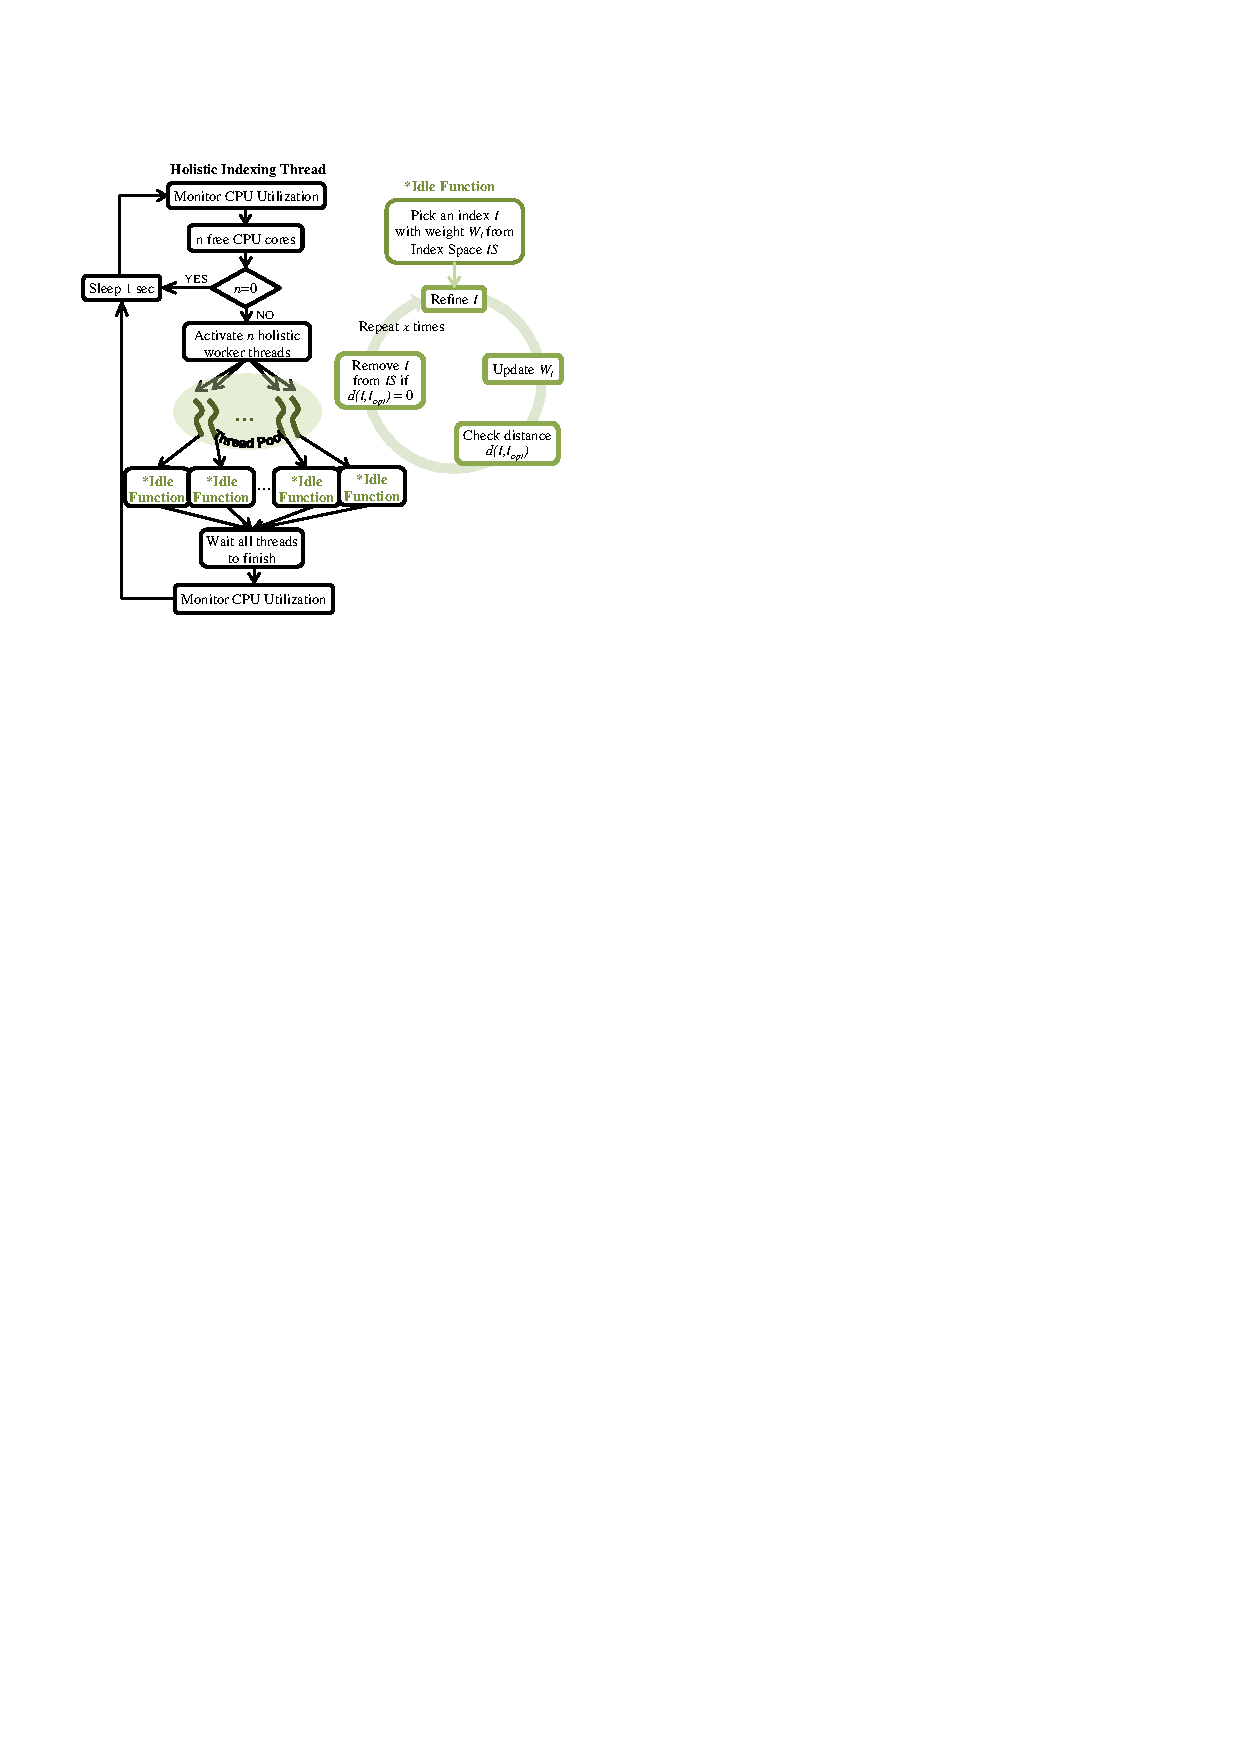
\includegraphics[trim=1.3cm 18.5cm 0cm 2.7cm]{Figures/holistic/diagram}
\vspace{-0.6 in}
\caption{Tuning actions.}
\vspace{-0.7 cm}
\label{fig:diagram}
\end{center}
\end{figure}

\textbf{Index Decision Strategies.} 
Another decision we have to make is which index to refine out of the pool of candidate indices.
Here, we describe four different strategies we can follow in order to pick an index from the index space.
The notion behind the first three strategies is that, since the only information we have is the past workload, 
we can exploit this information in order to prepare the physical design for a similar future workload.
On the contrary, the fourth strategy makes random choices.

For all strategies, a weight \emph{W$_{I}$} is assigned to each index \emph{I} in the index space.
When an index \emph{I} is added in the candidate indices, its weight is initialized 
to the distance between \emph{I} and \emph{I$_{opt}$}, which is given by Equation \eqref{eq:d}. 
For each index $I$, initially, there is only one partition (p$_{I}=1$) in \emph{I}, i.e., the entire column. 
Thus, the initial weight \emph{W$_{I_{init}}$} is equal to $N_{I} - L_{1_{s}}$,
where $N_{I}$ is the cardinality of the respective attribute (with type $T$) and $L_{1_{s}}$ is the number of elements of type $T$ that can fit into $L_{1}$ cache. 
The weight is used as a priority number in the first three strategies.
The index with the highest priority, i.e., the maximum weight,  in \emph{C$_{actual}$} is refined first.
When \emph{W$_{I}$} becomes equal to zero, \emph{I} is transferred 
from \emph{C$_{actual}$} to \emph{C$_{optimal}$} and it is not considered for further refinement in the future.
If \emph{C$_{actual}$} is empty, an index is randomly picked from \emph{C$_{potential}$}.
The weight of each index is constantly updated after every index refinement regardless of whether it is caused
by a user query or by holistic indexing.
Below we describe the four strategies.

\vspace{-0.2cm}
\begin{itemize}
  \setlength{\itemsep}{0cm}
  \setlength{\parskip}{0cm}
  \setlength{\parsep}{0cm}
\item \textbf{W1:} $W_{I}=d_{I}=d(I,$$I_{opt})$. Using this strategy, we give a priority to indices with large partitions.  
\item \textbf{W2:} $W_{I}=f_{I}*d_{I}$. Priority is given to indices that have large partitions and at the same time are accessed frequently in the workload. $f_{I}$ is the number of user queries that access $I$.
\item \textbf{W3:} $W_{I}=(f_{I}-f_{I_{h}})*d_{I}$. In this strategy we try to identify indices that are accessed frequently in the workload and at the same time have large partitions, because they have a high hit rate. These indices have a smaller priority compared to indices with large partitions that are accessed less frequently. $f_{I}$ is the number of user queries that access $I$, while $f_{I_{h}}$ is the number of user queries that do not trigger a refinement of $I$ because the requested value bound already exists in $I$.
\item \textbf{W4:} Make a random choice.
\end{itemize}
\vspace{-0.2cm}

Overall, our analysis, which is described later in Section~\ref{subsec:strategies} (Figure~\ref{fig:hvsc}), with numerous workloads showed
that even though small improvements can be achieved when picking the perfect strategy for each workload,
the random strategy gives a good and robust overall solution that is always close to the best for all workloads.
 
\begin{figure}
%\begin{center}
\hspace{3em}
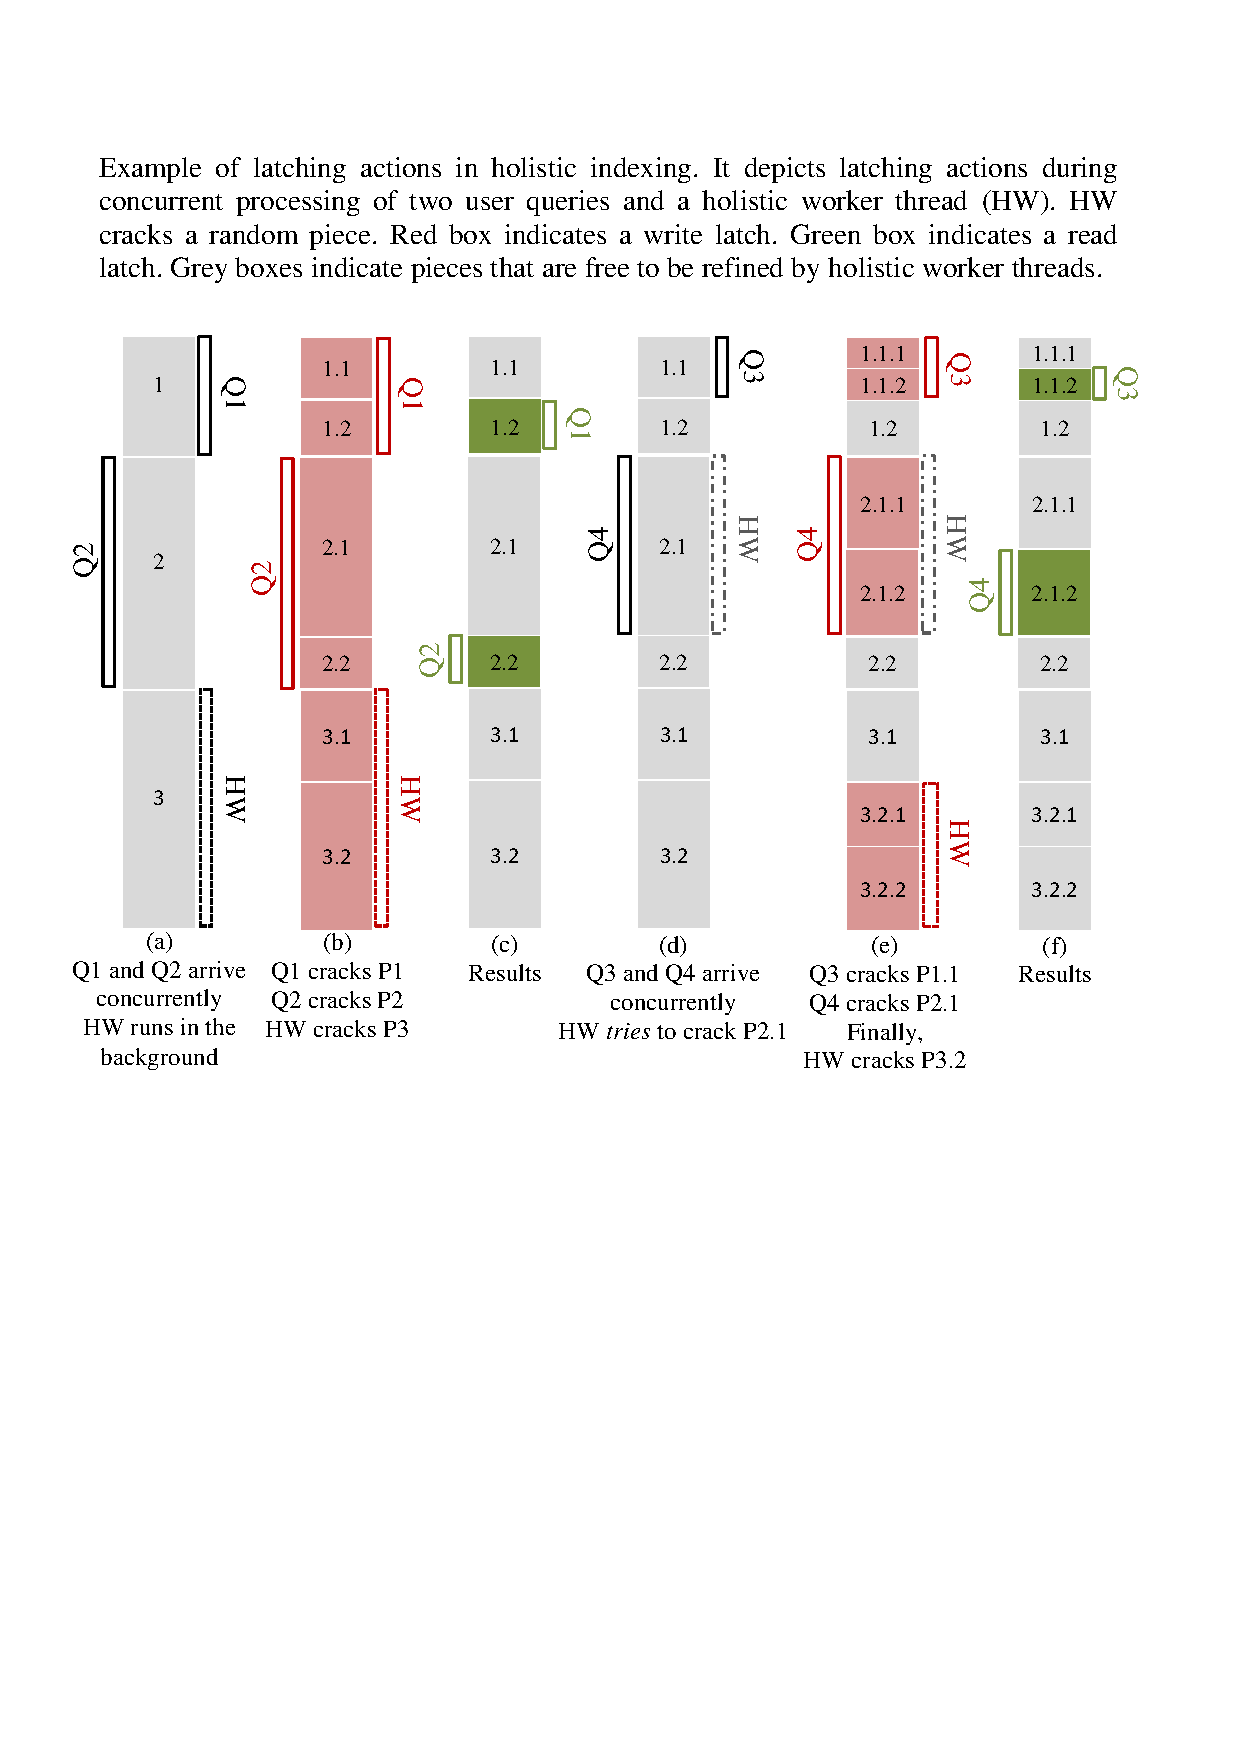
\includegraphics[trim=2.5cm 13cm 1.5cm 2.5cm,width=0.4\textwidth]{Figures/holistic/latching}
\vspace{0.5em}
\caption{Concurrency control in holistic indexing.}
\vspace{-0.4cm}
\label{fig:conc}
%\end{center}
\end{figure}
%\newpage
\textbf{Concurrency Control.}  
An index refinement due to holistic indexing happens in parallel with user queries.
Since user queries may also cause refinement of adaptive indices, we need to properly control
these changes. In addition, as more than one holistic thread may be active at any time, they may 
be trying to refine the same index. 
The study of concurrency control for adaptive indexing \cite{DBLP:journals/pvldb/GraefeHIKM12, DBLP:journals/vldb/GraefeHIKMS14} showed that it is possible to allow multiple
concurrent index refinements in adaptive indices via lightweight concurrency control, i.e., relying only on latches of individual pieces
in an adaptive index.
The point is that an index refinement only changes the structure of the index and not its contents (contrary to an actual update).
In this case, an index refinement only rearranges values in a single piece of a column at a time.
Thus it is sufficient to allow
other queries to work on different pieces in parallel by taking 
read/write latches on individual pieces, called piece latches in \cite{DBLP:journals/pvldb/GraefeHIKM12, DBLP:journals/vldb/GraefeHIKMS14}.
We exploit these techniques here in order to allow user queries and holistic workers to work concurrently over a single column, but
we also identify extra opportunities to increase parallelism for holistic workers.

Figure~\ref{fig:conc} shows an example of an adaptive index where two queries are actively cracking it.
Each query is interested in its own value range and needs to crack one piece, i.e., at the value of its selection.
The idea is that \emph{all} other pieces of the column are available for index refinement by holistic worker threads.
One direction would be that each holistic worker decides which piece of an index to refine
by picking from a list of pieces that currently have no locks.
However, such information is expensive to maintain similarly to our discussion in the ``Index Refinement'' paragraph.
Thus, holistic workers make random choices regarding which value to use as pivot and thus which piece to crack.
However, when a holistic worker requests a write latch to crack a piece and it happens that the piece is locked at the moment, then 
if the latch is not given immediately, the worker picks another random pivot and repeats the procedure
until it finds a free piece to crack. In contrast, user queries need to always block in such cases and wait for the piece to be unlocked.
For instance, in Figure~\ref{fig:conc}(d) the holistic worker thread tries to lock piece 2.1, which is already locked by Q4.
Instead of waiting for the lock to be released, the worker chooses another pivot.
The new pivot falls in piece 3.2, which is not locked and it is reorganized finally by the worker (Figure~\ref{fig:conc}(e)).
As we process more queries and as we perform more holistic indexing, 
the number of pieces in an index grows; as a side-effect 
the waiting time for taking a latch decreases as there are more candidate pieces to pick from.


\textbf{Updates.} 
Updates for adaptive indexing have been studied in \cite{DBLP:conf/sigmod/IdreosKM09}.
The design in \cite{DBLP:conf/sigmod/IdreosKM09} is that updates remain as pending updates
and are merged during query processing, i.e., if a query requests a value range that contains one or more pending updates,
then only those updates are merged on-the-fly and without destroying any of the information on the adaptive index.
Each query needs to lock at most one column piece at a time for cracking and can update this piece at the same time if pending updates for this piece exist \cite{DBLP:journals/pvldb/GraefeHIKM12, DBLP:journals/vldb/GraefeHIKMS14}. Multiple queries may work in parallel updating and cracking separate pieces (value ranges) of the same column.

The difference here is that with holistic indexing, holistic workers not only perform
auxiliary index refinement actions but also merge pending updates.
That is, if a holistic worker picks a pivot which falls within a piece of the respective column and the value range,
for which this piece holds values, has pending updates, then all those pending updates are merged by the holistic worker.
In this way, holistic worker threads not only refine the adaptive indices in the background but also bring them 
more up to date which removes further load from future queries.

\begin{figure}[!t]
\begin{center}
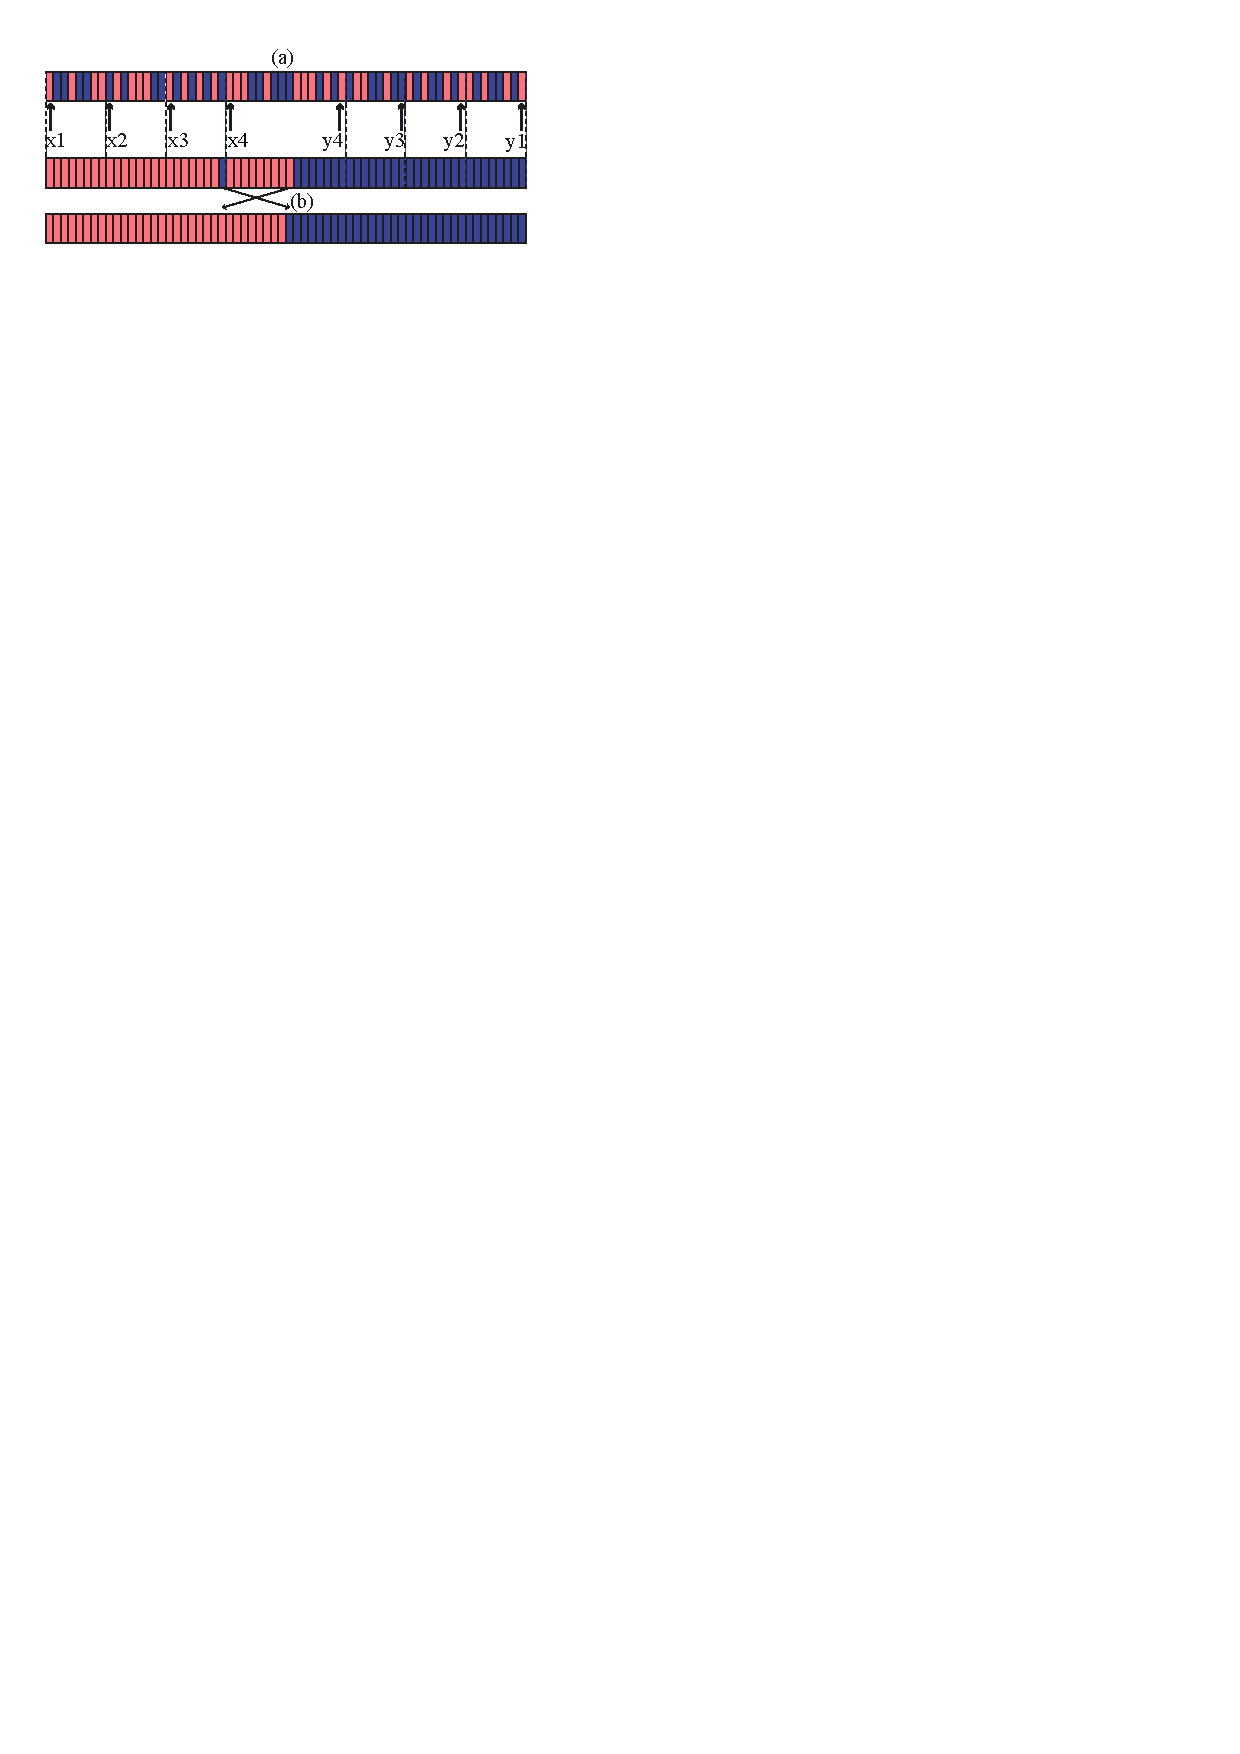
\includegraphics[trim=-0.5cm 25.7cm 0.5cm 1cm,width=2\columnwidth, height=1.8cm]{Figures/holistic/mcrack2}
\vspace{-0.25 in}
\caption{Refined Partition \& Merge (multi-threaded) \cite{efficient_cracking}.}
\vspace{-0.7cm}
\label{fig:mt-cracking}
\end{center}
\end{figure}

\begin{figure}[!t]
\begin{center}
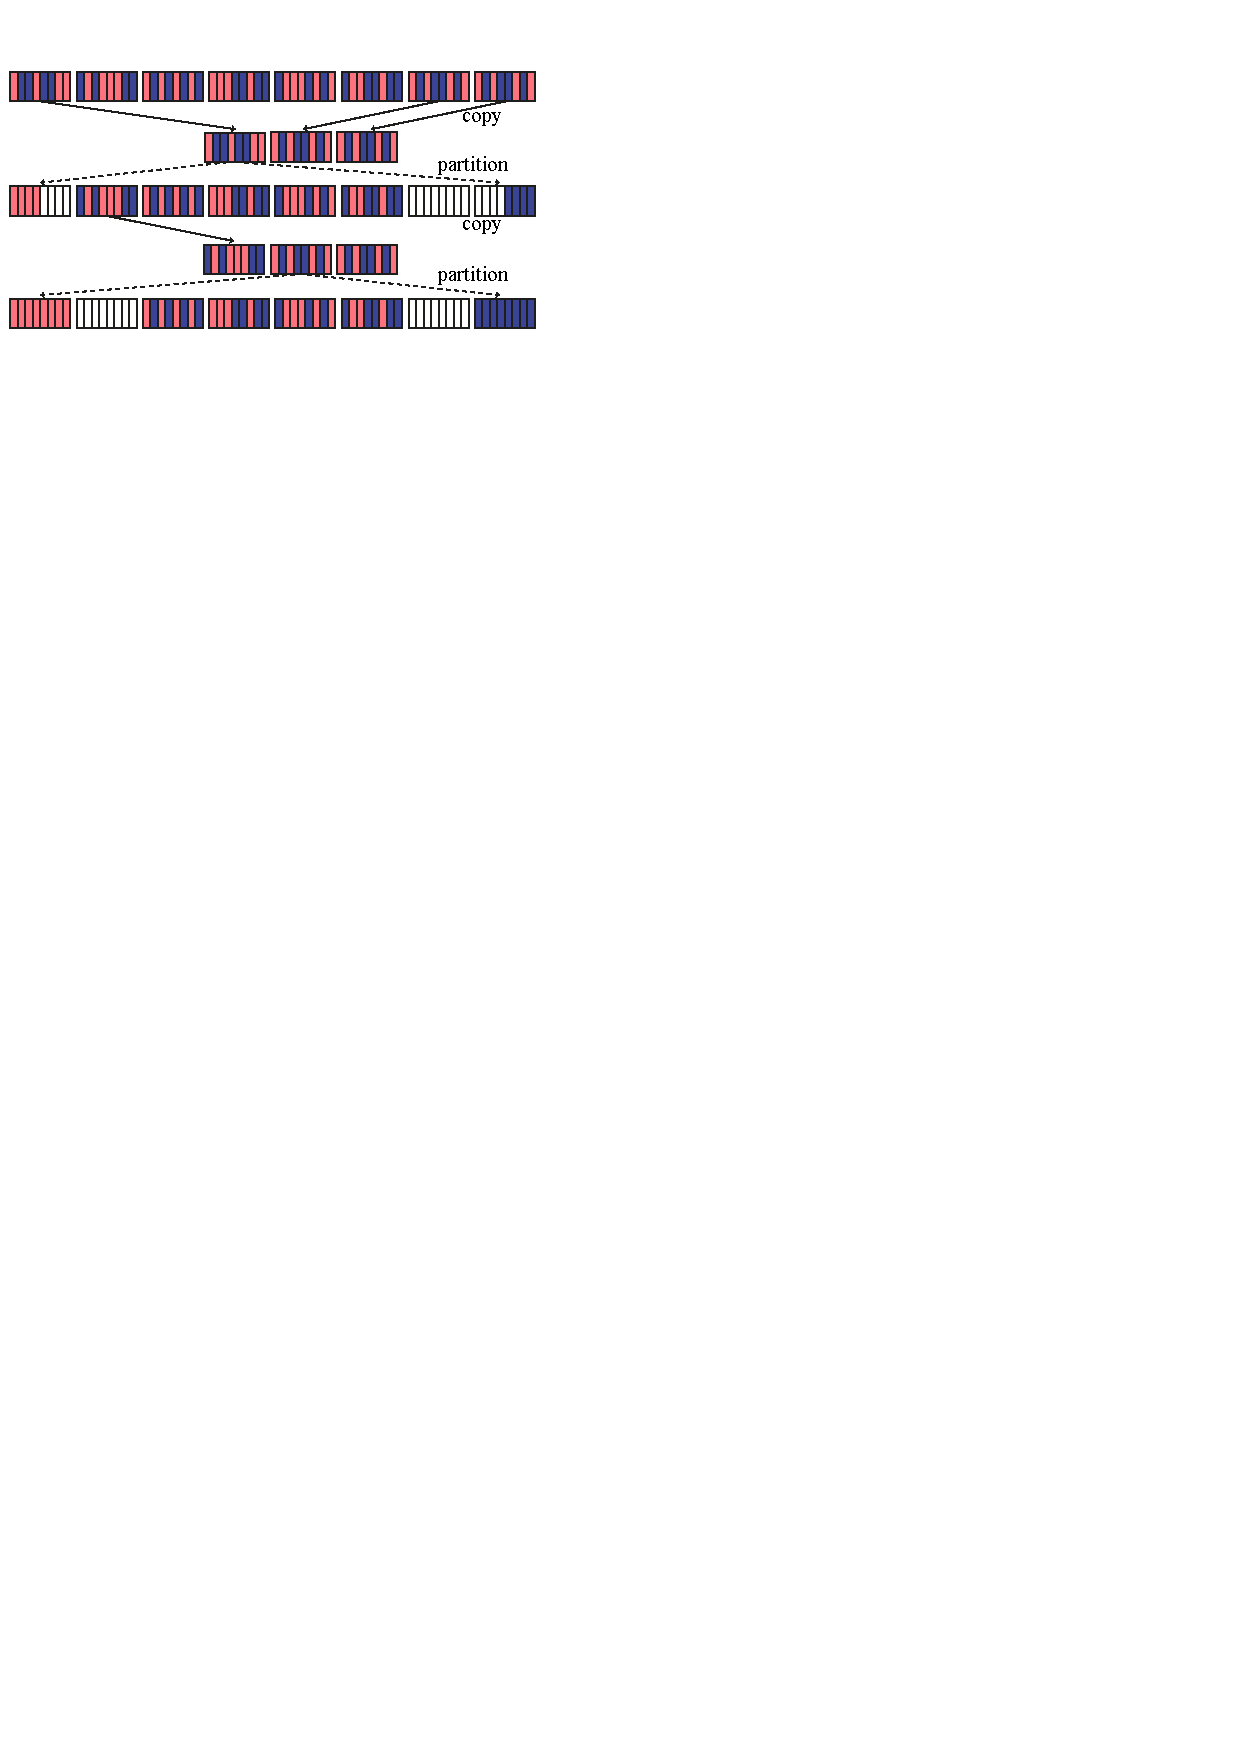
\includegraphics[trim=0cm 24.5cm 0cm 1cm,width=2.3\columnwidth,height=2.8cm]{Figures/holistic/vectorized}
\caption{Vectorized Cracking \cite{efficient_cracking}.}
\label{fig:vectorized-cracking}
\vspace{-0.7cm}
\end{center}
\end{figure}

\begin{figure*}[!t]
     \begin{center}
	 \subfloat[Performance]{%
	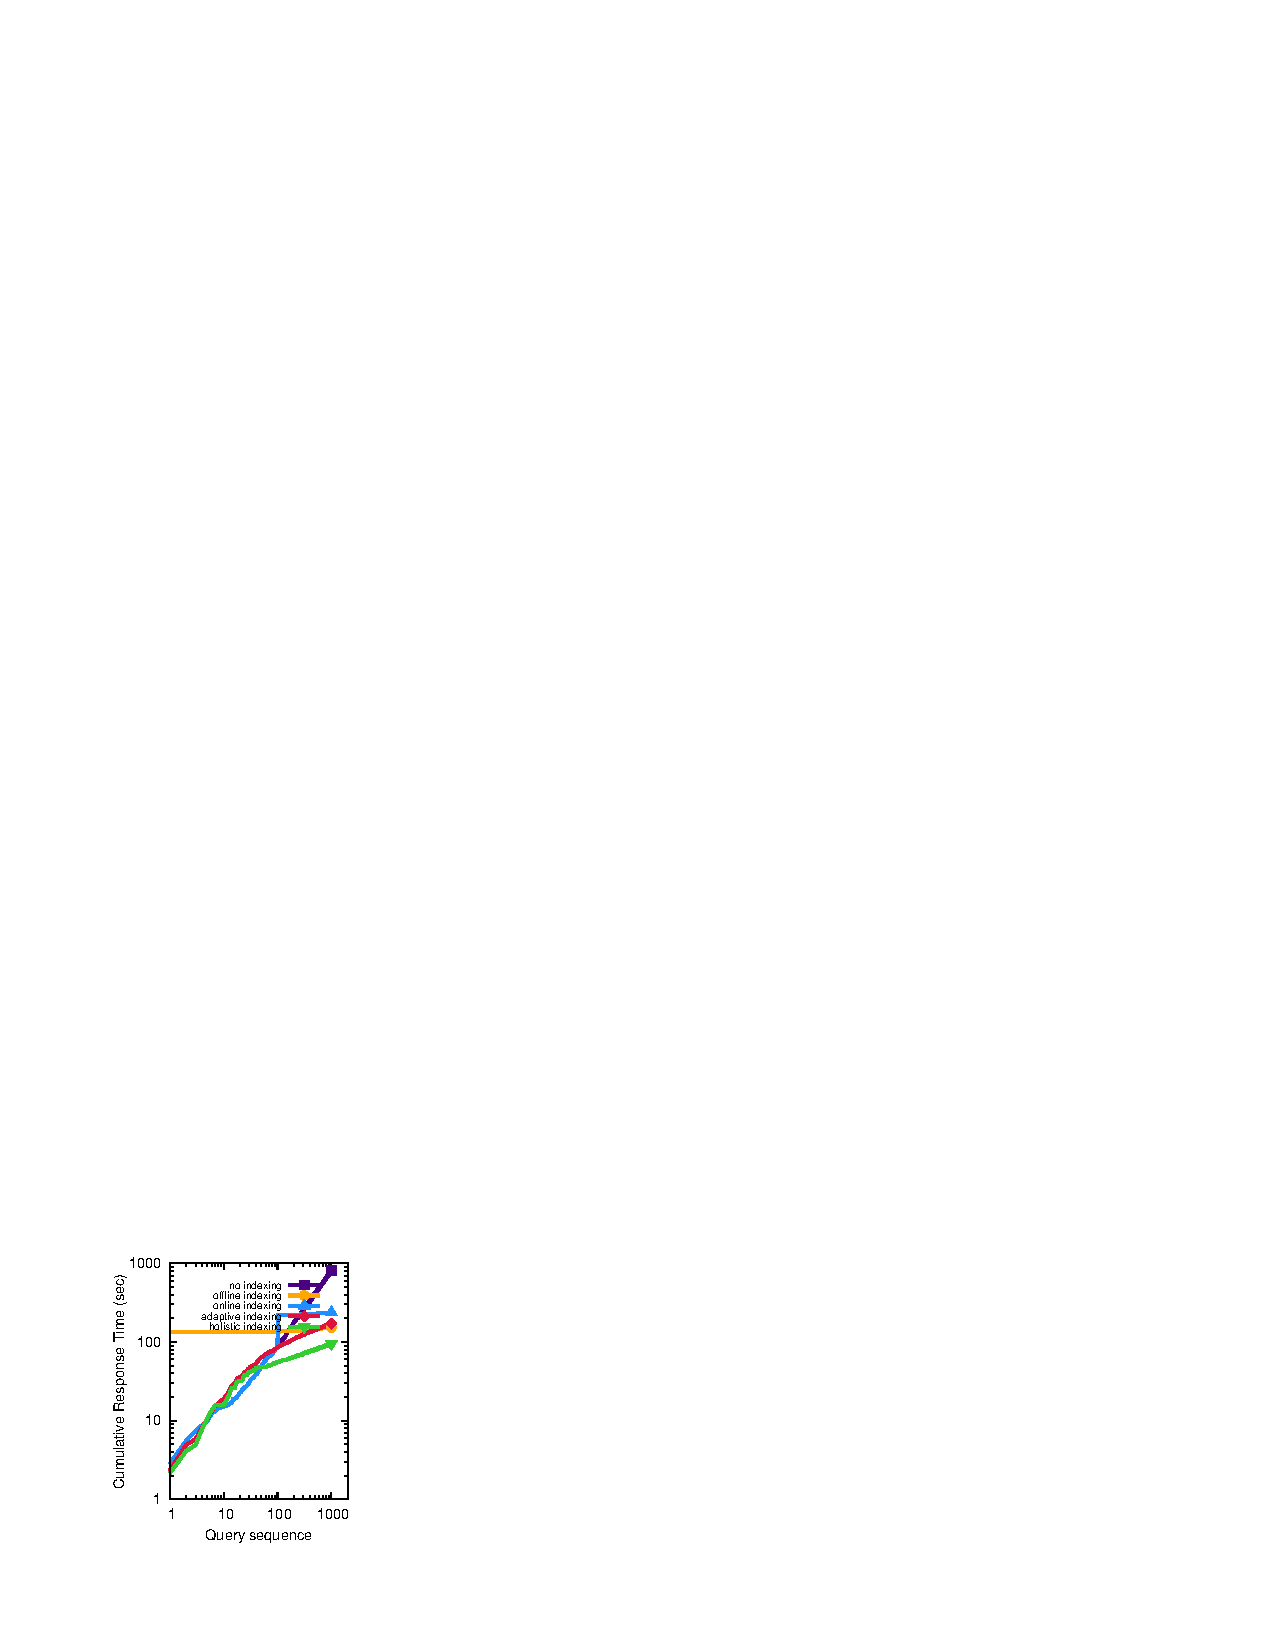
\includegraphics[trim=2cm 2.2cm 15cm 21.7cm]{Figures/holistic/motivation}
	}%
	 \subfloat[Performance Breakdown]{%
	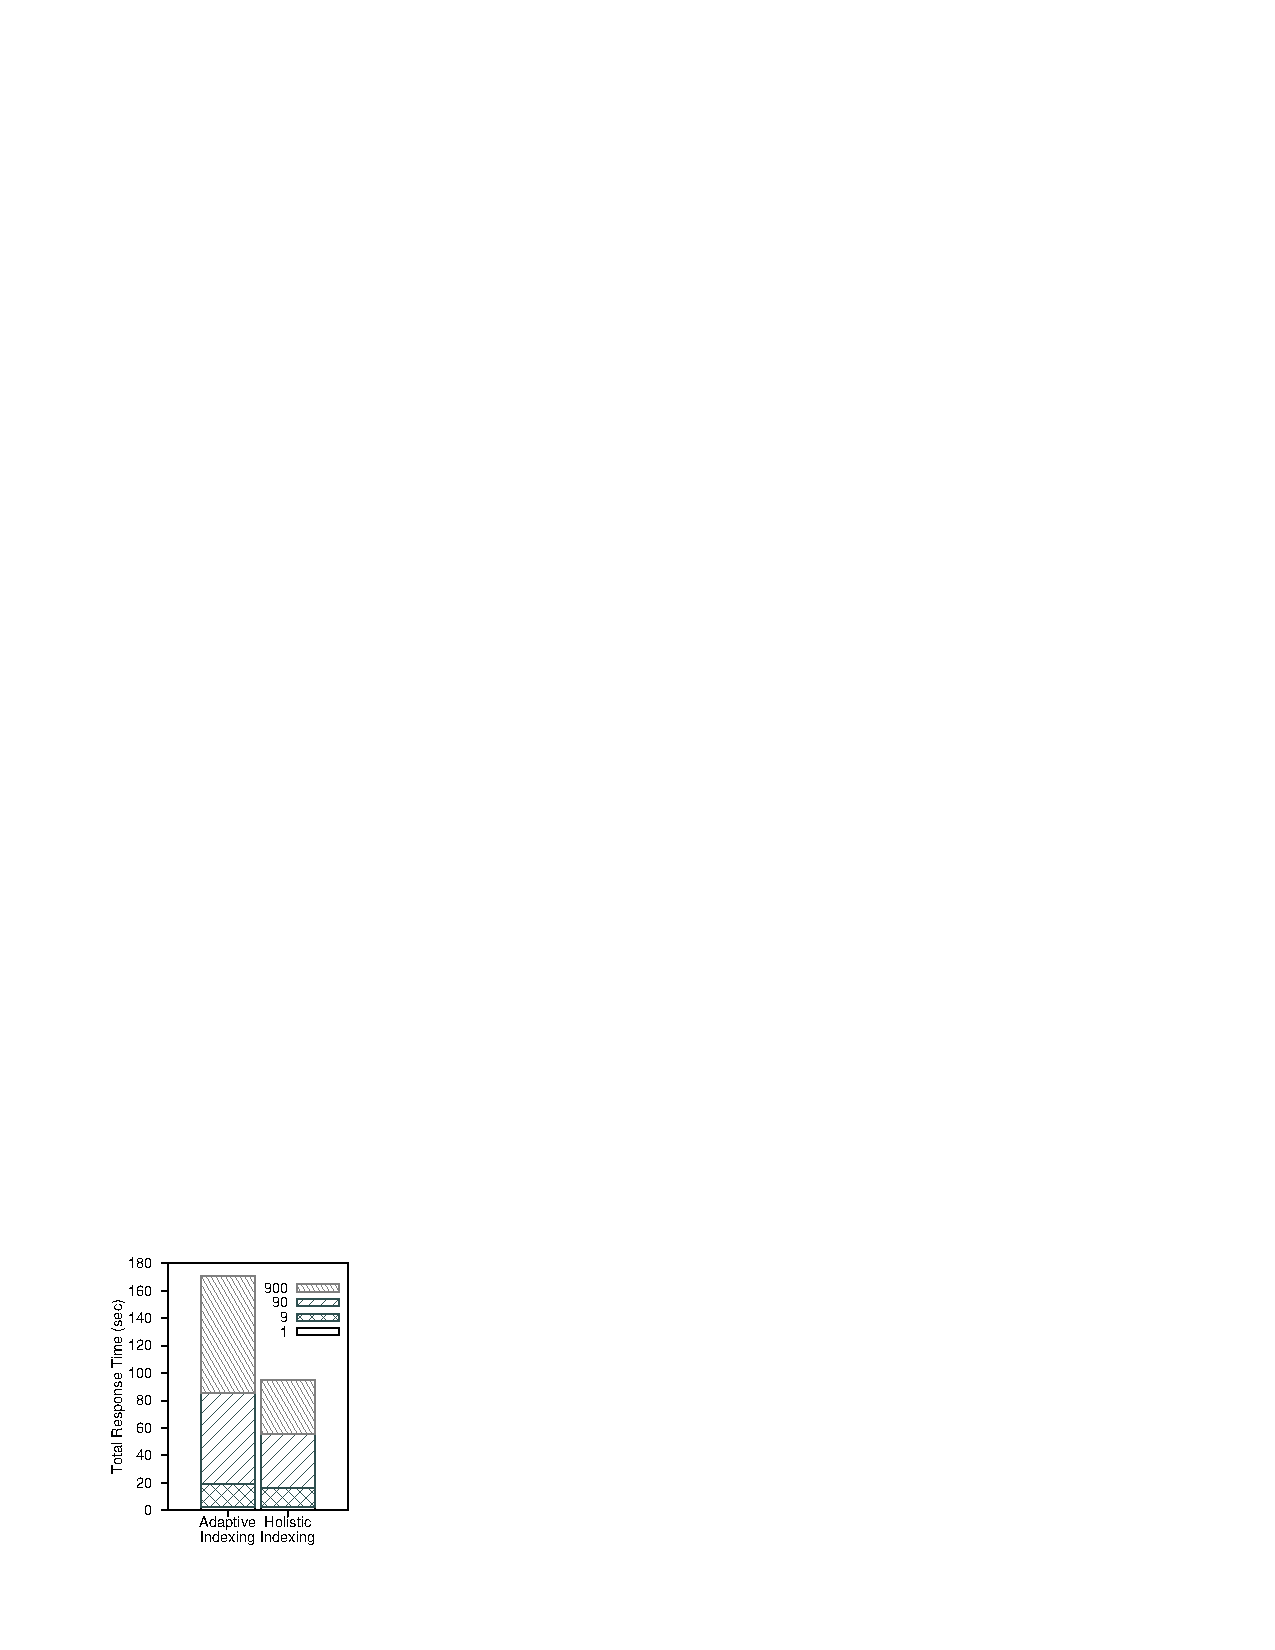
\includegraphics[trim=2.3cm 2.1cm 15cm 21.7cm]{Figures/holistic/hist_motivation}
	}%
	 \subfloat[Index Partitions]{%
	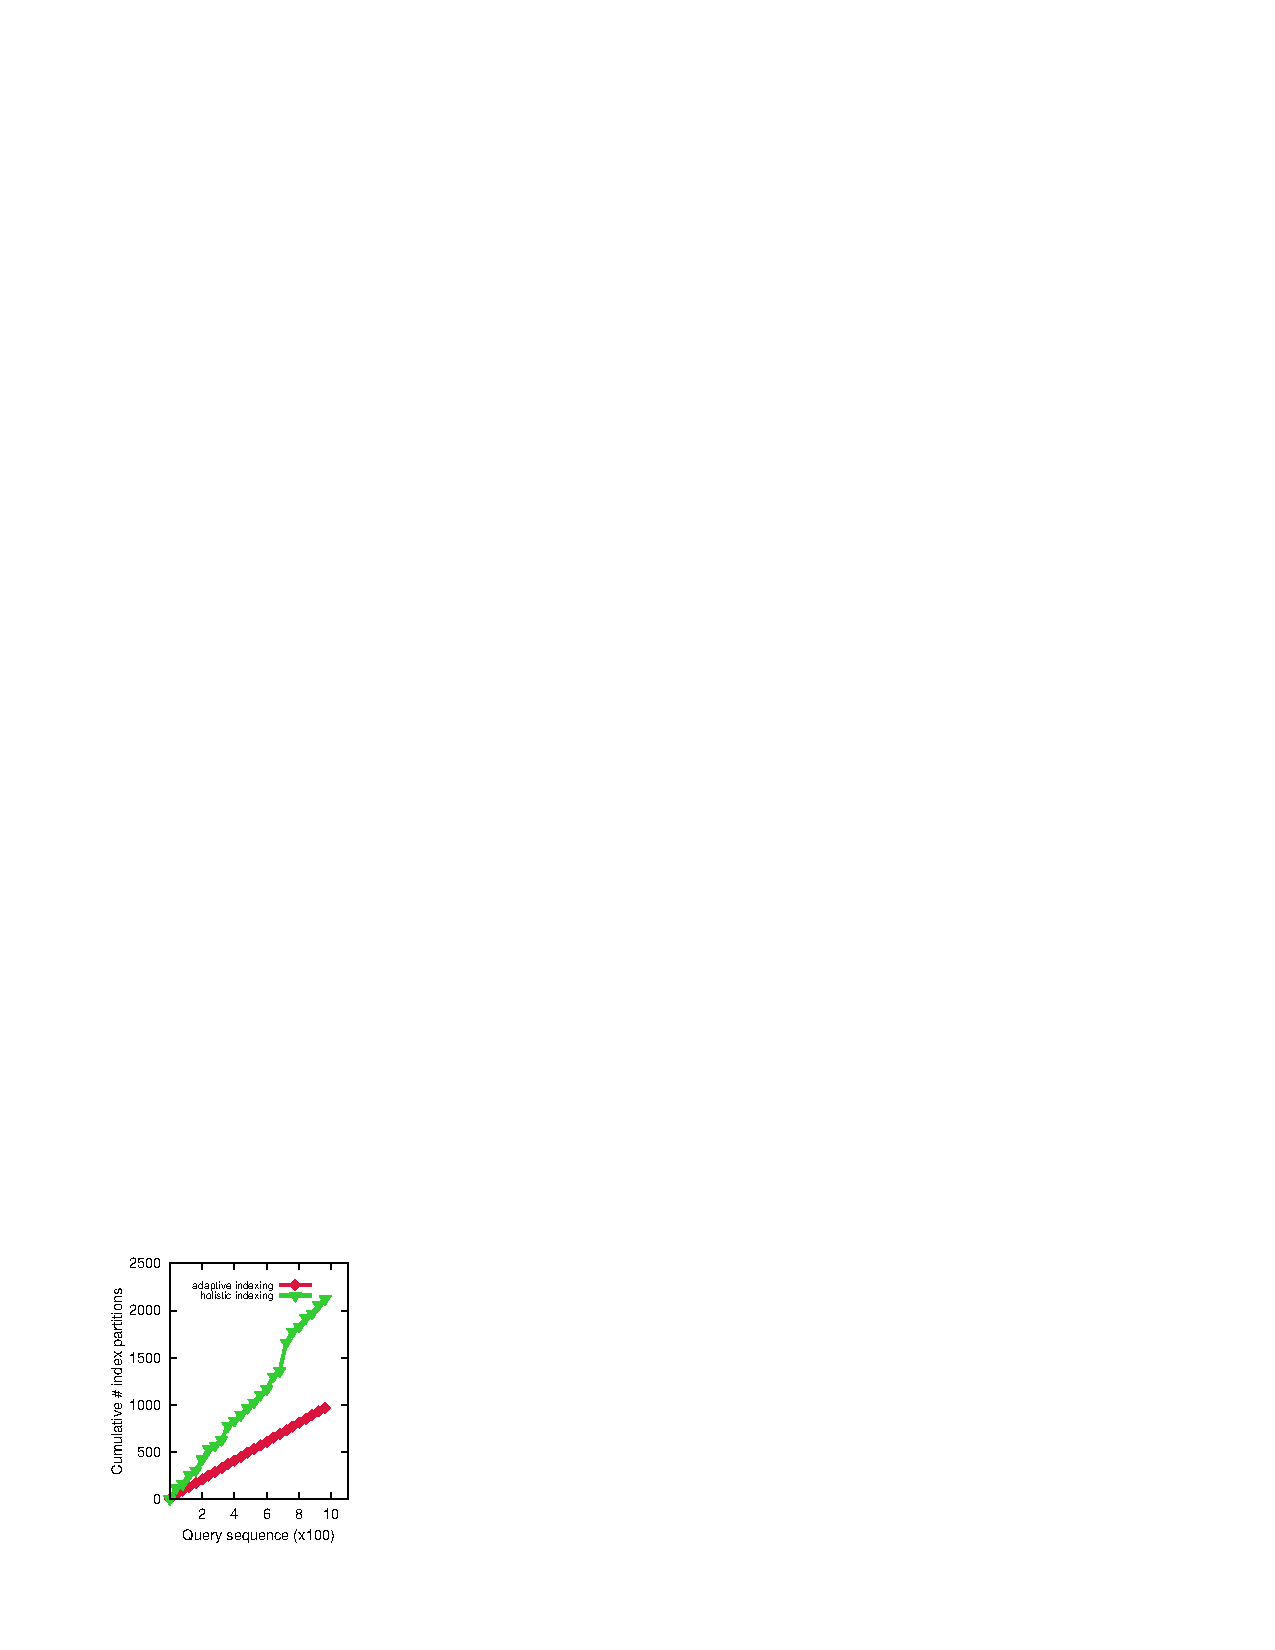
\includegraphics[trim=2.3cm 2.2cm 15cm 21.7cm]{Figures/holistic/pieces_motivation}
	}%
	 \subfloat[Idle CPU Utilization]{%
	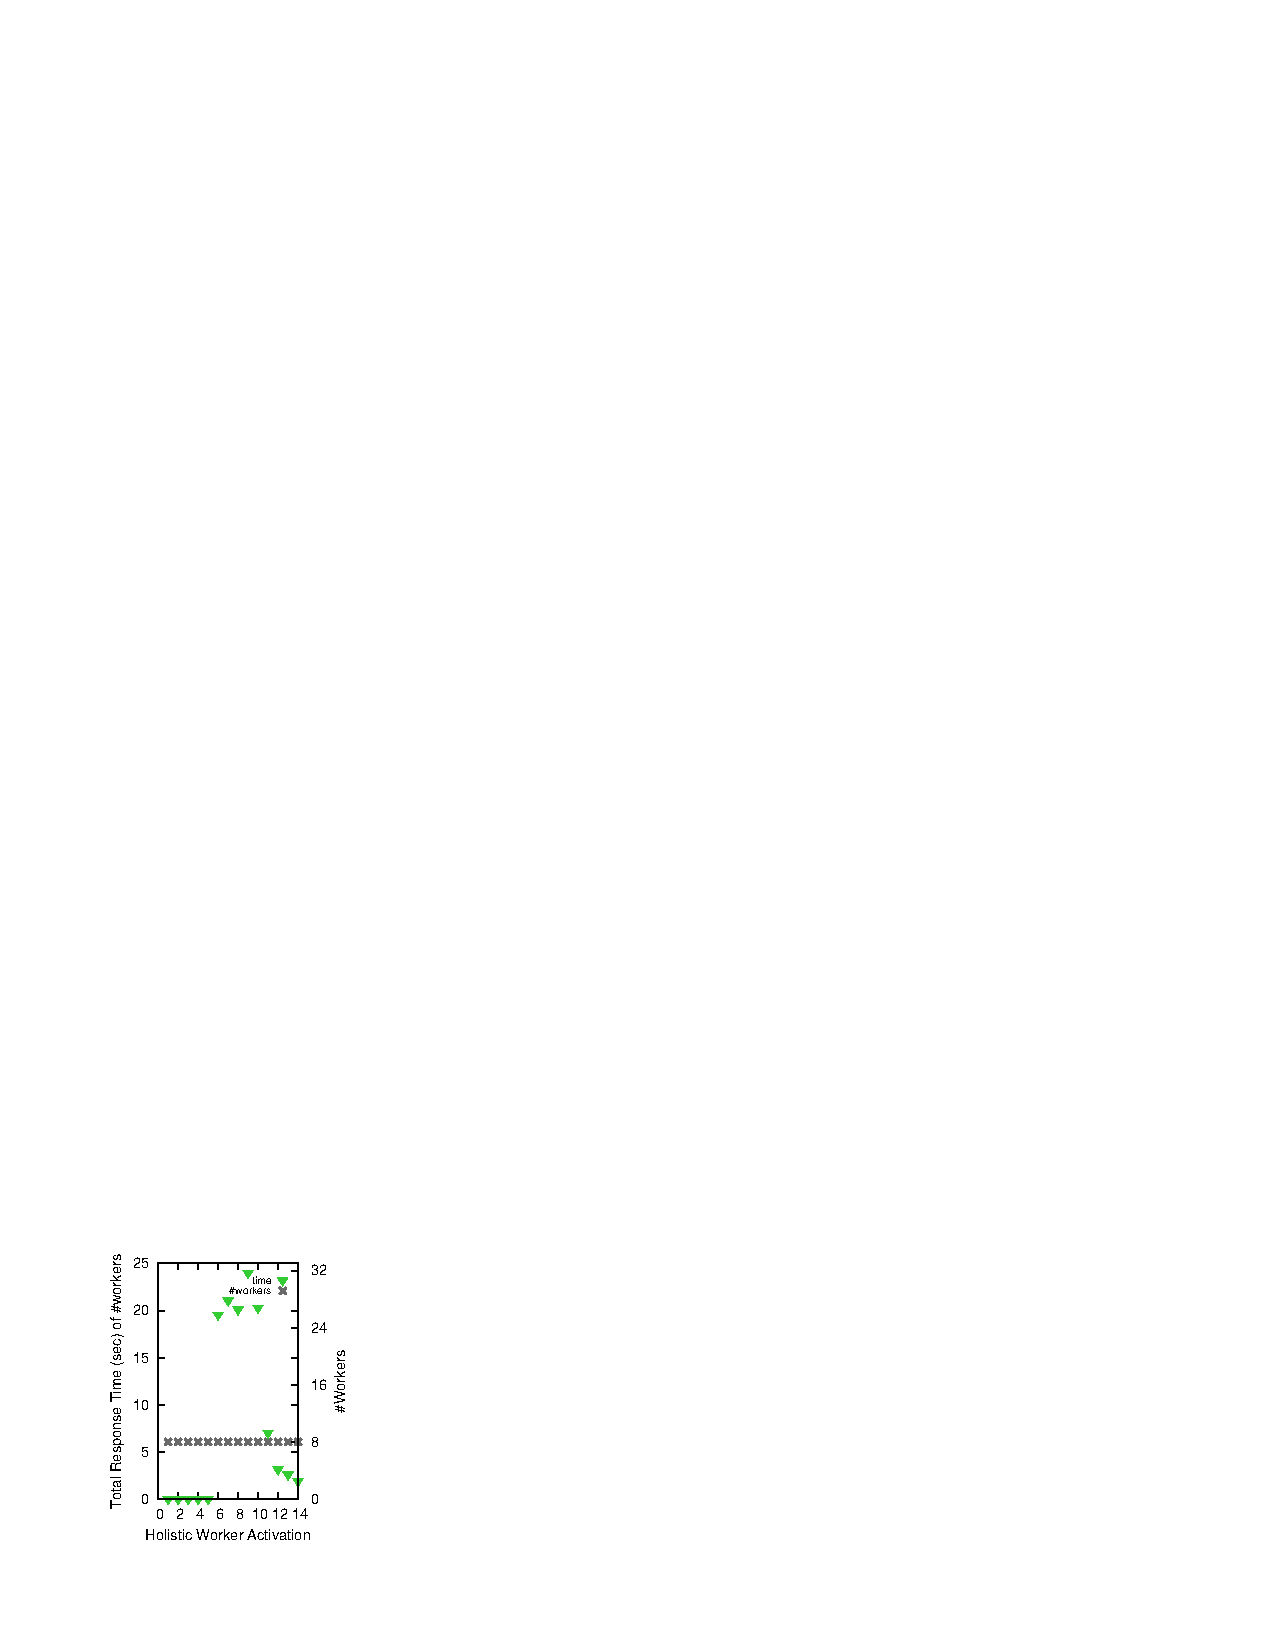
\includegraphics[trim=2cm 2.2cm 15.5cm 21.7cm]{Figures/holistic/workers}
	}%
	\vspace{-0.25 in}
	\caption{Improving performance with holistic indexing.}
	\vspace{-0.7 cm}
	\label{fig:motiv}
     \end{center}%\end{figure*}
\end{figure*}

\textbf{Storage Constraints.} 
Holistic indexing works within a limited storage budget.
Adaptive indices may be dropped or recreated at any time. 
They consist auxiliary information and thus dropping an index does not lead to any loss of data.
In case the storage budget does not allow adding a new index triggered by a user query, 
then indices are removed with a least frequently used (LFU) policy from the index space
at an index-level granularity or at a fine-grained granularity that allows for creating and dropping individual ranges dynamically, as partial cracking suggested in \cite{DBLP:conf/sigmod/IdreosKM09}.

\textbf{Multi-core Adaptive Indexing.}
The goal of holistic indexing is to improve the physical design by fully utilizing the available CPU resources.
An alternative approach to achieve maximum CPU utilization is to parallelize the index refinement actions triggered by user queries.
This problem was studied in \cite{efficient_cracking}, which introduced a multi-core, CPU efficient cracking algorithm shown in Figure~\ref{fig:mt-cracking}.
In this algorithm, the to-be-cracked piece is partitioned initially into as many slices as the number of threads, e.g., $n$ (Figure~\ref{fig:mt-cracking}(a)).
The center slice is contiguous, while the
remaining $n-1$ slices consist of two disjoint halves, each, that are arranged
concentrically around the center slice ($x_{i}$ and $y_{i}$ indicate the first and the last element of piece $i$ respectively).
$n$ threads crack the $n$ slices independently applying a vectorized, out-of-place cracking algorithm (Figure~\ref{fig:vectorized-cracking}), which was proven  in 
\cite{efficient_cracking} to be the most CPU efficient single-threaded cracking implementation reported so far.
Finally, the local data are merged into a big cracked piece (Figure~\ref{fig:mt-cracking}(b)).
We found that devoting all resources to perform adaptive indexing for user queries in parallel does not lead to the absolute best performance. 
Specifically, we found that we can improve performance even more by assigning part of the resources to holistic indexing. 
In this way, some of the CPU resources are assigned to parallel cracking for user queries but the rest of the CPU resources
are distributed across several holistic workers for additional index refinements.
In the experimental section we show why this approach is better than assigning all available resources to user queries.


